\documentclass[tikz,border=2pt]{standalone}
\usepackage{amsmath,amssymb}
\usepackage{pgfplots}
\pgfplotsset{compat=1.18}

\begin{document}
% Exponential densities for rates 1 and 2: the density starts at lambda and decays
% exponentially; a larger rate means shorter waiting times (mean 1/lambda).
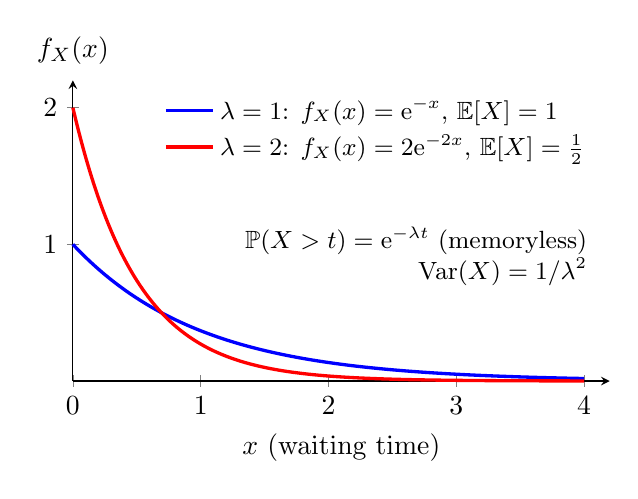
\begin{tikzpicture}
	\begin{axis}[
		axis lines=left, xmin=0, xmax=4.2, ymin=0, ymax=2.2,
		xtick={0,1,2,3,4}, ytick={1,2},
		xlabel={$x$ (waiting time)}, ylabel={$f_X(x)$}, ylabel style={rotate=-90, anchor=south, at={(axis description cs:0,1.02)}},
		samples=120, smooth, width=8.4cm, height=5.4cm, clip=false,
		legend style={draw=none, fill=none, font=\small}, legend cell align=left
		]
		\addplot[blue, very thick, domain=0:4] {exp(-x)};
		\addlegendentry{$\lambda=1$: $f_X(x)=\mathrm{e}^{-x}$, $\mathbb{E}[X]=1$}
		\addplot[red, very thick, domain=0:4] {2*exp(-2*x)};
		\addlegendentry{$\lambda=2$: $f_X(x)=2\mathrm{e}^{-2x}$, $\mathbb{E}[X]=\tfrac12$}
		\node[anchor=north east, font=\small, align=right] at (axis cs:4.1,1.2) {$\mathbb{P}(X>t)=\mathrm{e}^{-\lambda t}$ (memoryless)\\ $\operatorname{Var}(X)=1/\lambda^2$};
	\end{axis}
\end{tikzpicture}
\end{document}
